% !TEX encoding = UTF-8 Unicode
% -*- coding: UTF-8; -*-
% vim: set fenc=utf-8

\chapter{Arquitetura ARMFUL}%
\label{chap:arquitetura-armful}

Nesse capítulo será apresentada a arquitetura \abbrev{ARMFUL}{Analysis of Raw Data from Multiple Files} ARMFUL (do inglês: Analysis of Raw Data from Multiple Files; em tradução livre: Análise de Dados Científicos de Múltiplos Arquivos), introduzida recentemente em~\cite{silva2016situ,silva2017raw} pelo laboratório de \abbrev{NACAD}{Núcleo Avançado de Computação de Alto Desempenho} Núcleo Avançado de Computação de Alto Desempenho (NACAD) da \abbrev{UFRJ}{Universidade Federal do Rio de Janeiro} UFRJ (Universidade Federal do Rio de Janeiro). Também será abordado o \textit{DfAnalyzer}, uma instância dessa arquitetura, implementada pelo mesmo laboratório.

\section{Visão geral}

A \textbf{arquitetura ARMFUL} tem suporte a extração de dados científicos, a técnicas de indexação e a análise de dados científicos a partir de múltiplos arquivos~\cite{silva2016situ} com o propósito de permitir o acesso direto a qualquer elemento ou região específica do espaço do fluxo de dados de uma simulação científica. Em outras palavras, ela permite a execução, \textit{off-line} e~/~ou \textit{on-line}\footnote{\textit{I.e.}, as consultas podem ser realizadas tanto \emph{após} as simulações científicas, quanto \emph{durante} as mesmas, respectivamente.}, de todos os três tipos de consultas apresentadas na \autoref{sec:tipos-de-consulta}. Essa flexibilidade e versatilidade na análise existe graças a uma \textbf{arquitetura de componentes}, que utiliza um banco de dados de proveniência para proporcionar um caminho de acesso entre o fluxo de dados e os dados científicos~\cite{silva2017raw}.

% Baseado na seção 5 de~\cite{silva2017raw}. Tentativa de tradução livre e de adaptação para o contexto desse trabalho.
A arquitetura ARMFUL funciona do seguinte modo: a gerência de conteúdos científicos é obtida a partir de dados científicos de arquivos, que então são correlacionados, em um repositório que é um SGBD relacional, através de dados de proveniência do seu respectivo fluxo de dados. Essa gerência de dados requer características que são específicas do domínio da simulação científica; por isso, modelos de dados de proveniência dessas simulações costumam ser representados em granularidade não-fina, \textit{i.e.}, as tabelas do SGBD possuem um grau de abstração relativamente alto para representar esses dados. Entretanto, consultas de proveniência possuem um valor analítico limitado caso não sejam relacionadas a elementos de dados específicos ao domínio da simulação computacional; contudo, esse relacionamento exige bastante esforço dos usuários de SGWfCs no que diz respeito a desenvolver, para cada domínio, um modelo de dados e programas científicos específicos para acessar, extrair e correlacionar os dados de domínio aos dados de proveniência. Nesse aspecto, a arquitetura ARMFUL contribui diminuindo o esforço necessário para capturar e representar esses dados de proveniência aravés da introdução e divisão de componentes genéricos e auto-contidos que modelam e correlacionam entre si, no mesmo banco de dados, (\(i\)) dados científicos específicos do domínio e (\(ii\)) proveniência.

Na \autoref{fig:armful-architecture-simplified}, podemos visualizar como é feita a representação e a divisão em componentes da arquitetura ARMFUL, que são os seguintes:

\begin{itemize}
    \item Banco de dados de proveniência;
    \item Extração de dados científicos;
    \item Indexação de dados científicos;
    \item Ingestão de dados de proveniência; e
    \item Processamento de consultas.
\end{itemize}

\begin{figure}[ht]
    \centering
    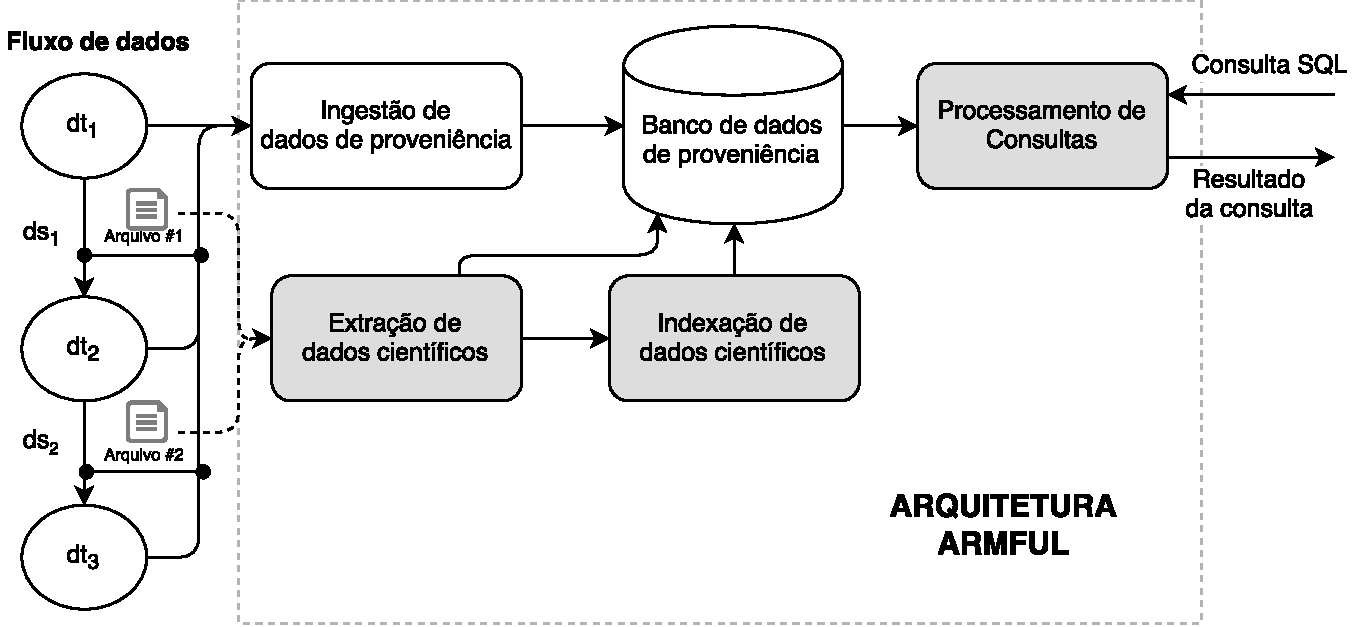
\includegraphics[width=\textwidth]{img/armful-architecture-simplified}
    \caption[Componentes da arquitetura ARMFUL]{Componentes da arquitetura ARMFUL. A cor branca representa as etapas relacionadas à proveniência de dados, e a cor cinza tem relação com os dados científicos. Baseada em~\cite{silva2017raw}.}%
    \label{fig:armful-architecture-simplified}
\end{figure}

Os componentes na cor branca correspondem à captura e ao armazenamento de dados de proveniência em um banco de dados de proveniência. Em contrapartida, os componentes na cor cinza descrevem os passos responsáveis por: (\(i\)) extrair dados científicos de arquivos, (\(ii\)) gerar índices para os mesmos e (\(iii\)) permitir a consulta de proveniência \textbf{e} dados científicos a partir do mesmo banco de dados. Nas próximas subseções os componentes serão detalhados.

% Baseado na seção 5.1 de~\cite{silva2017raw}.
\subsection{Banco de dados de proveniência}%
\label{subsec:banco-de-dados-de-proveniencia}

O \textbf{banco de dados de proveniência}, que funciona como um repositório para os dados de proveniência, deve ser um \textbf{SGBD relacional}, e é responsável por armazenar, gerenciar e correlacionar (\(i\)) dados de proveniências e (\(ii\)) dados científicos, a fim de se beneficiar do suporte analítico de consultas do fluxo de dados. Além disso, SGBDs possuem solidez, confiabilidade e segurança, oriundas de uma experiência de mais de 30 anos de estudos científicos e aplicações no mundo real, provendo estratégias e algoritmos bem conhecidos que garantem atomicidade, consistência, isolamento e durabilidade (ACID) em transações, além de possuir soluções consolidadas e robustas no que diz respeito a recuperação de dados e controle concorrente de acesso~\cite{ozsu2011principles}.

\subsection{Extração e indexação de dados científicos}

O \textbf{componente de extração de dados científicos} tem o objetivo de ler o conteúdo de arquivos científicos, analisá-lo e então recuperar parte do conteúdo selecionado que é relevante de acordo com os atributos especificados pelo usuário. Para que esse objetivo seja completado, quatro etapas devem ser seguidas:

\begin{itemize}
    \item \textbf{leitura do conteúdo}: acesso aos arquivos científicos e leitura do seu conteúdo;
    \item \textbf{tokenização}: investigação de metadados relacionados à especificação do formato de arquivo, visando verificar se os dados científicos obtidos na etapa anterior correspondem ao domínio da simulação computacional processada atualmente;
    \item \textbf{filtragem de conteúdo}: a especificação do usuário é responsável por definir e restringir o que deve ser analisado e armazenado no banco de dados de proveniência, isto é, essa etapa evita armazenar atributos desnecessários, que não serão utilizados na próxima etapa;
    \item \textbf{análise}: conversão de cada dado científico filtrado em uma estrutura de dados apropriada para ser armazenada no SGBD.
\end{itemize}

O \textbf{componente de indexação de dados científicos} é opcional e visa indexar um conteúdo específico dos arquivos científicos a fim de agilizar o tempo de acesso direto a determinadas regiões do espaço de dados científicos através da gerência de metadados correlacionados ao fluxo de dados. A criação de índices é realizada segundo um algoritmo de indexação previamente definido, \textit{e.g.} indexação por \textit{bitmap} ou indexação posicional.

O volume de dados científicos que é gerado durante a execução de uma simulação computacional é um fator determinante para a definição da melhor estratégia para a representação desses dados~\cite{silva2015propostadoutorado}: em simulações que geram um pequeno volume de dados em cada transformação de dados e que possuem poucos atributos, a extração e ingestão (\textit{i.e.}, carga no banco de dados de proveniência) de dados científicos \emph{diretamente} com seus próprios valores de dados costuma ser uma abordagem melhor. Em contrapartida, em um cenário no qual um grande volume de dados --- com estruturas de dados complexas --- precisa ser capturado, o componente de indexação é fortemente recomendado.

\subsection{Ingestão de dados}

O \textbf{componente de ingestão de dados} é responsável por coletar a \textbf{proveniência} do fluxo de dados, selecionando, manipulando e armazenando (\textit{i.e.} realizando a carga dos valores assumidos pelos atributos) convenientemente as informações referentes aos arquivos e dados científicos no banco de dados mencionado na \autoref{subsec:banco-de-dados-de-proveniencia}~\cite{silva2015propostadoutorado}. Em outras palavras, esse componente é responsável por alimentar e popular o SGBD com informações de proveniência de dados que serão posteriormente utilizadas para auxiliar o componente de processamento de consultas, que será discutido na próxima seção. Esse componente interfaceia diretamente com todo item do fluxo de dados.

A captura de dados de proveniência deve ser realizada com uma granularidade fina, de modo a apoiar e capturar os dois tipos de análises exploratórias em arquivos de dados científicos mencionadas na \autoref{subsec:categorias-de-dados-de-proveniencia} (proveniência prospectiva e retrospectiva). Além disso, também deve realizar a gerência do fluxo de dados nos níveis físico e lógico.

\subsection{Processamento de consultas}

Uma vez que todos os dados científicos e toda a proveniência sejam devidamente capturadas e armazenadas em um repositório SGBD, os usuários poderão consultá-los para apoiar (refutar ou validar) suas hipóteses científicas~\cite{silva2015propostadoutorado}. Nesse contexto, o \textbf{componente de processamento de consultas} é responsável por prover um mecanismo de consultas à proveniência e aos dados científicos armazenados em um banco de dados de proveniência compatível com um modelo de dados adequado. O comportamento desse componente é variável, dependendo da estratégia utilizada nos componentes anteriores --- de extração e de indexação. Uma vez que esse componente utiliza um SGBD para o armazenamento dos dados de proveniência, somente tipos de consultas que são permitidas e disponíveis pelo SGBD podem ser realizadas. Em particular, e como consequência disso, as consultas são comumente especificadas em uma linguagem de alto nível, como a linguagem declarativa SQL.

O processador de consultas é um componente bastante importante, já que é a principal interface entre os usuários e uma instância da arquitetura ARMFUL, e todas as consultas ao banco de dados são iniciadas (e especificadas) a partir dele.

\section{DfAnalyzer: uma instância da arquitetura ARMFUL}

Como vimos na seção anterior, a arquitetura ARMFUL é uma \textbf{abstração} que define e especifica componentes a fim de prover um mecanismo capaz de realizar consultas a um banco de dados de proveniência oriundo de uma simulação computacional. Dito isso, o \textbf{DfAnalyzer} é uma \textbf{instância} da arquitetura ARMFUL; em outras palavras, é um exemplo de implementação e uso da mesma para um contexto e uma aplicação de simulação de dinâmica computacional de sedimentação de fluidos. Ele foi originalmente introduzido em~\cite{silva2016situ}.

\perrotta{TODO: EXPAND. SuperComputing, 2017, 2015}

\subsection{Provenance Data Gatherer (PDG)}

O Provenance Data Gatherer (PDG), 

% Provenance Gatherer (origem da proveniência para o banco de dados que eu vou utilizar na QueryProcessor)

\perrotta{TODO: EXPAND}

\subsection{Raw Data Extractor (RDE)}

\perrotta{TODO: EXPAND}

\subsection{Raw Data Indexer (RDI)}

\perrotta{TODO: EXPAND}

\subsection{Query Processor (QP)}

\perrotta{TODO: EXPAND}
\perrotta{TODO: to mention my contribution}

% QueryProcessorCaptura de dados de proveniência}